\chapter{Background}
\label{chapter2}
\thispagestyle{plain}

 In Section \ref{sec:relevant_methodologies_used} we will go through software development methodologies used to assess the requirements. The methodologies mentioned in \ref{sec:relevant_methodologies_used} hep us create a framework upon which we build our solution.

\section{Relevant Methodologies Used}\label{sec:relevant_methodologies_used}


\subsection{Agile Software Development}
Agile \footnote{https://www.agilealliance.org} software development is an umbrella term for a set of frameworks and practices based on the values and principles expressed in the Manifesto for Agile Software Development.

Agile by nature focuses on customer collaboration, interactions between individual members of a development team, and most importantly responding to unforeseen changes (that may arise during development cycle) in requirements. The goal of agile is to produce a working software rather than a comprehensive documentation.

Some of the more famous agile based frameworks are as follows:
\begin{itemize}
  \item Scrum
  \item Rapid application development(RAD)
  \item lean software development
  \item lean startup
  \item feature driven development
  \item extreme programming(XP)
\end{itemize}
We chose Scrum for the purpose of this project and throughout \ref{sec:scrum_methodology} we describe how it works.

The Agile software development life cycle is an iterative process. Each iteration delivers a piece of working software available for use by the customer until the final product is complete. The duration of each iteration is usually two to four weeks in length and by definition has a fixed completion time. 
As it is evident due to the iterative nature of Agile software development life cycle, multiple iterations take place during development, with each iteration completed the customers and business stakeholders provide additional feedback in order to ensure the features delivered meet their requirements.


Figure \ref{fig:agile_pic_cycle} illustrates a typical iteration process flow of agile methodology. Each iteration is composed of phases which are described briefly below:
\begin{enumerate}
  \item Requirements: Define the requirements for the iteration based on the product backlog, sprint backlog, customer and stakeholder feedback.
  \item Design \& Development: Design and develop software based on defined requirements.
  \item Testing: QA (Quality Assurance) testing, internal and external training, documentation development.
  \item Deployment: Integrate and deliver the working iteration into production.
  \item Review: Accept customer and stakeholder feedback and work it into the requirements of the next iteration.         
\end{enumerate}

\begin{figure} 
\centering
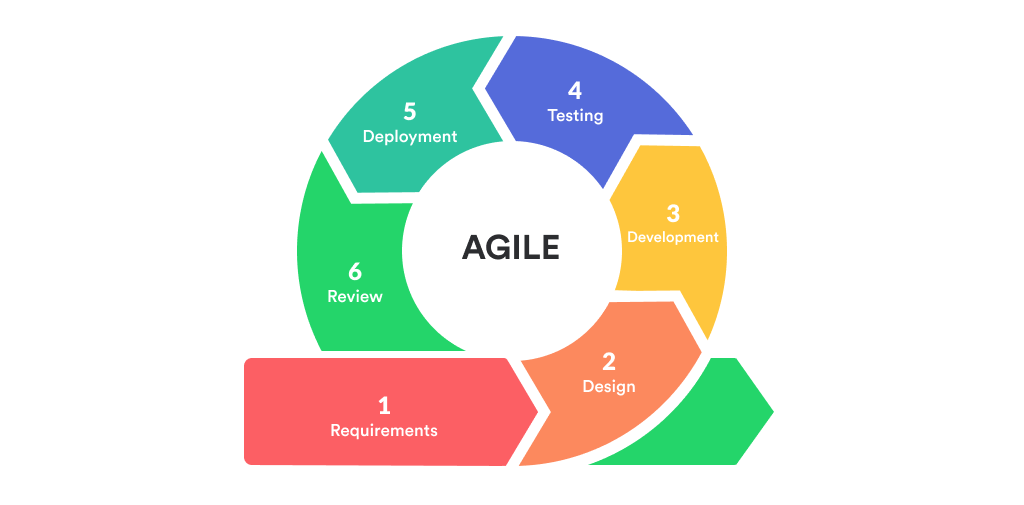
\includegraphics[width=16cm]{pictures/agile_pic.png}
\caption{Agile Framework}
Figure illustrating phases of an iteration in Agile methodology.
\label{fig:agile_pic_cycle}
\end{figure}

\subsection{Scrum}
\label{sec:scrum_methodology}
Scrum \footnote{https://www.scrum.org} is an agile process framework for managing complex knowledge work, with an initial emphasis on software development. 
We choose Scrum because it is adaptive,it uses iterative cycles, and it is fast and flexible therefore this methodology allows us to deliver significant value to the customer early on. Scrum ensures transparency in communication and creates an environment of collective accountability and continuous progress. 

We start by gathering information about the product and the requirements in form of User Stories.
A user story is the smallest unit of work in an agile framework. It is an end goal, not a feature, expressed from the software users perspective. User stories are usually developed through discussions with stakeholders.
A common template for a user story is as follows:
As a\textless role\textgreater I can\textless capability\textgreater, so that\textless receive benefit\textgreater.
User stories are grouped together in order to from Epics. Epics are a collection of user stories which are related to each other either implicitly or explicitly.
The scrum team usually choose epics based on a list of prioritized requirements defined by the customer. The chosen epics enter the product backlog\footnote{https://www.scrum.org/resources/what-is-a-product-backlog}.
In scrum, the Product Backlog is an ordered list of everything that is known to be needed in the product. It is the single source of requirements for any changes to be made to the product.
The scrum team identifies a list of tasks from the product backlog, these tasks must be completed by the end of the Scrum Sprint.
Sprint\footnote{https://www.scrum.org/resources/what-is-a-sprint-in-scrum} is a time-box of one month or less during which a “Done”, usable, and potentially releasable product Increment is created. 

\begin{figure} 
\centering
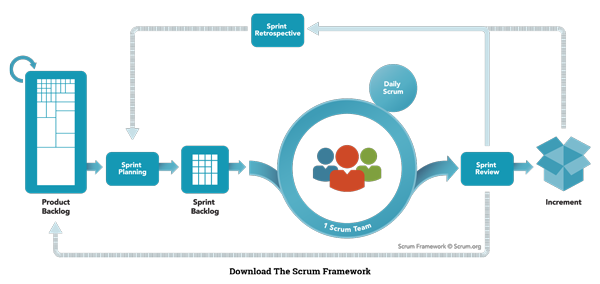
\includegraphics[width=14cm]{pictures/Scrum_Framework.png}
\caption{Scrum Methodology}
Figure illustrating various phases of scrum methodology. 
\label{fig:scrum_pic}
\end{figure}


\section{Relevant Technologies} \label{sec:relevant_technologies}
In this section we introduce technologies used for the development of this project. Figure \ref{fig:taxonomy} shows the main elements of our web application. We will go through main elements of proposed architecture for our web application in section \ref{sec:three_tier}. Once we defined the architecture we plan to use, in section \ref{sec:spring_web} we will discuss the technology used for the front-end and finally in \ref{sec:ext_js} the back-end platform of choice is examined.



\begin{figure} 
\centering
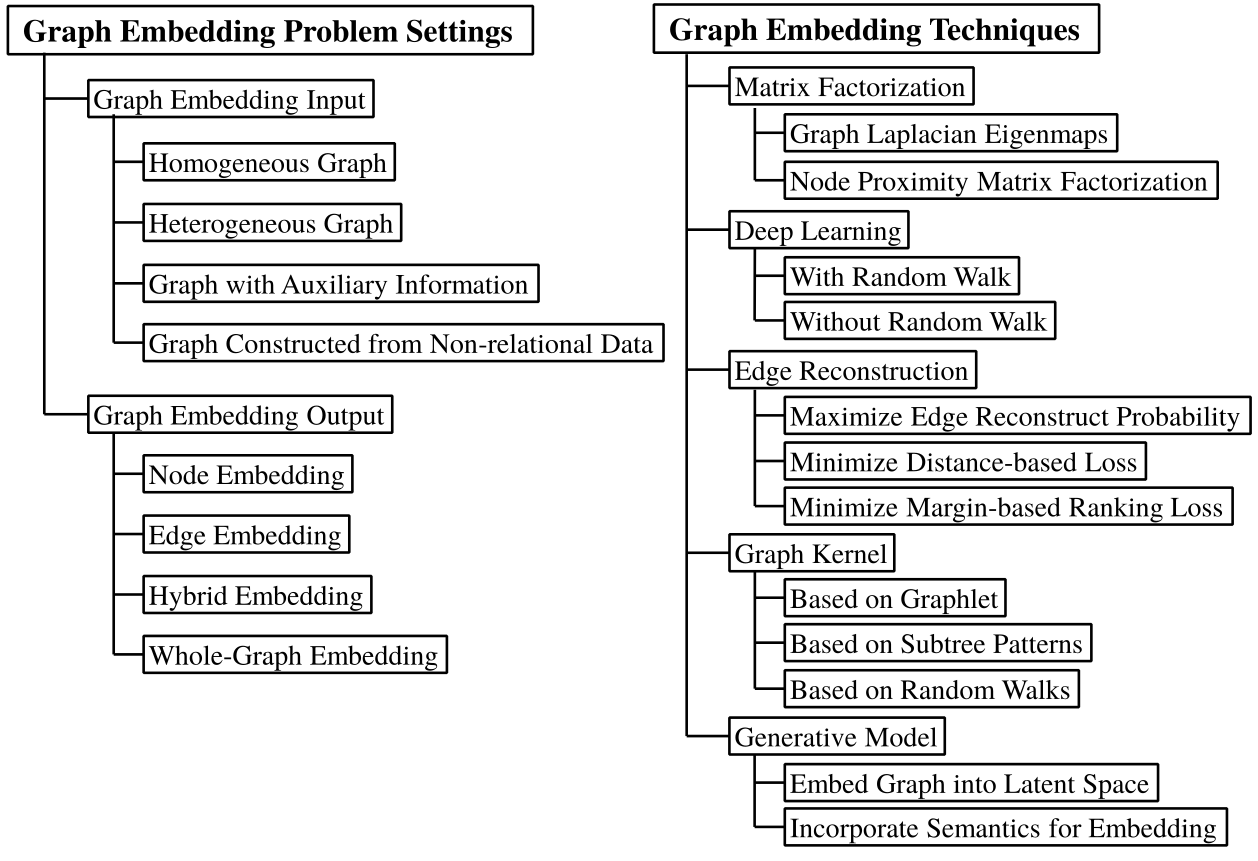
\includegraphics[width=8cm]{pictures/taxonomy.png}
\caption{Model for Web application}
Figure illustrating main elements of our web application and how they work together.
\label{fig:taxonomy}
\end{figure}

\subsection{Three tier architecture}
\label{sec:three_tier}
In this section we will examine our proposed architecture for the application, which is three tier architecture.

The three tier architecture is a client-server architecture, in which tier represents physical separation and layer represents logical separation.
In this architecture each layer can potentially run on a different machine. In addition each tier is developed and maintained as independent modules, most often on separate platforms. 

Some aspects concerning design of three tier architecture are as follows:
\begin{itemize}
    \item Unconnected tiers should not communicate.
    \item Change in platform affects only the layer running on that particular platform. 
    \item Data transfer between tiers is part of the architecture. Protocols involved may include one or more of SNMP, CORBA, Java RMI, .NET Remoting, Windows Communication Foundation, sockets, UDP, web services or other proprietary protocols.
    \item Three tier architecture follows component-oriented approach, generally the architecture uses platform specific methods for communication instaed of a message based approach.
\end{itemize}


Now we briefly discuss role of each tier and how tiers work together. Figure \ref{fig:three_tier_pic} illustrates elements discussed below.
\begin{enumerate}
    \item \textbf{Presentation Tier/Front-end:}  
    This is the topmost level of the application.
    It provides user interface, handles the interaction with the user. Sometimes called the GUI or client view or front-end.
    It sends content to browsers in the form of HTML/JS/CSS. This tier may use frameworks such as React, Angular, Ember, Aurora, etc.
    It communicates with business logic tier in form of http request/response, which business logic tier can handle.
    \item \textbf{Application Tier/Back-end (Business Logic or Middle Tier):}
    This tier contains set of rules for processing information(business logic) and is able to accommodate many users. This tier is sometimes also called as middle-ware.
    Middle-ware processes the inputs received from the clients and interacts with the database.
    The logic tier will have the JSP, Java Servlets, Ruby, PHP, C++, Python and other programs. The logic tier runs on a Web server.
    \item \textbf{Data Tier:}
    A database, comprising both data sets and the database management system or RDBMS \footnote{Relational Database Management System} software that manages and provides access to the data (back-end).
    It provides security, data integrity and support application.
    The data tier is usually a kind of database, such as a MySQL, SQLite or PostgreSQL database running on a server.
\end{enumerate}
   

Now that we have defined the three tier architecture and how it works, we discuss the main advantages as well as disadvantages of using this architecture.

\textbf{Advantages:}
\begin{itemize}
    \item \textbf{Maintainability:}
    Because each tier is independent of the other tiers, updates or changes can be carried out without affecting the application as a whole.
    \item \textbf{Scalability:}
    Because tiers are based on the deployment of layers, scaling out an application is reasonably straightforward.
    \item \textbf{Flexibility:}
    Because each tier can be managed or scaled independently, flexibility is increased.
    \item \textbf{Availability:}
    Applications can exploit the modular architecture of enabling systems using easily scalable components, which increases availability.
    \item \textbf{Re-usability:} 
    Components are reusable
    \item \textbf{Faster development:}
    Because of division of work web designer does presentation, software engineer does logic, DB admin does data model.
\end{itemize}
   
\textbf{Disadvantages:}   
\begin{itemize}
    \item \textbf{Cost:} High installation cost.
    \item \textbf{Complexity:} Structure is more complex as compare to 1 \& 2 tier architectures.
\end{itemize}

\begin{figure} 
\centering
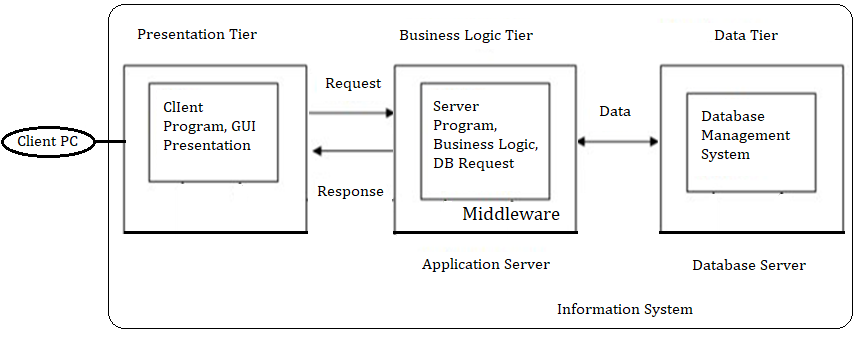
\includegraphics[width=14cm]{pictures/three-tier.png}
\caption{Taxonomy of three tier architecture}
Figure illustrating the three tier architecture. 
\label{fig:three_tier_pic}
\end{figure}


The usage of Cloud environments as Database solution provider is optimal for our architecture. The dynamic distributed database over Cloud Environment improves accessibility and response time for our clients as well as providing scalability in case of future expansions of our digital platform. Figure \ref{fig:taxonomy} illustrates this concept.

%We expand the concepts previously mentioned by adding another layer to the proposed architecture in order to further separate business-logic tier and data tier by adding API Server in the middle. The added level abstraction is specially useful for dynamic distributed database over Cloud Environment, API server simply contacts a database based on predetermined logic written for the specific API.
%For example one API server can request guest information from a database which only handles guest table requests, while another API is handling booking process and the database can be located on Cloud. 



%databases located on cloud servers possibly through distribute  
%The concepts previously mentioned 



\subsection{Spring for Web applications}
\label{sec:spring_web}
The Spring Framework is an application framework and inversion of control container for the Java platform. 

There are a few key concepts which need declaration.
Firstly we explain the concept of "Web Container" briefly. A Web Container is a java application that controls servlet. 
Servlets do not have a main() method, therefore they require a container to load them. In essence A Web Container is a place where servlets are deployed. Figure \ref{fig:request_pic} shows a request made by a client to the application server, when a client sends a request to the web server which contains a servlet, the web server redirects that request to the container rather than to the servlet directly. Figure \ref{fig:respond_pic} shows the response received by the client. In this case the Web Container finds out the servlet which requested a response and passes the Http Request as well as the response to the servlet and loads the servlet methods i.e. doGet() or do Post(). 
\begin{figure} 
\centering
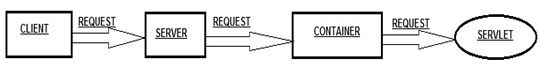
\includegraphics[width=14cm]{pictures/request_pic.jpeg}
\caption{Request from Client to Server}
Figure illustrating a request made by a client toward the web application server. 
\label{fig:request_pic}
\end{figure}
\begin{figure} 
\centering
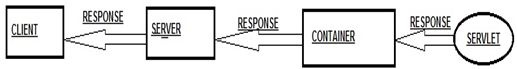
\includegraphics[width=14cm]{pictures/response_pic.jpeg}
\caption{Response from Server to Client}
Figure illustrating server response to the client request.
\label{fig:respond_pic}
\end{figure}

Secondly we introduce the concept of "Inversion of Control".
IOC \footnote{https://docs.spring.io/spring/docs/3.2.x/spring-framework-reference/html/beans.html\#beans-introduction} is a process whereby objects define their dependencies, that is, the other objects they work with,only through constructor arguments, arguments to a factory method, or properties that are set on the object instance after it is constructed or returned from a factory method.The container then injects those dependencies when it creates the bean.
In other words Inversion of control indicates the control flow of the program is inverted meaning that the control flow of the program is delegated to an external source, a.k.a. the container.

In addition the Spring IoC container consumes a form of configuration metadata which can be seen in figure \ref{fig:spring_ioc_container_pic}; this configuration metadata represents how an application developer instructs the Spring container to instantiate, configure, and assemble the objects in an application. Configuration metadata is traditionally supplied in a simple and intuitive XML format provided by the programmer.

\begin{figure} 
\centering
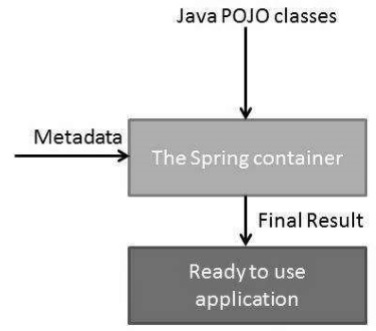
\includegraphics[width=8cm]{pictures/spring_ioc_container.jpg}
\caption{Spring container dependency injection}
Figure illustrating usage of user supplied Metadata and JAVA POJO classes for the purpose of dependency Injection into the application.
\label{fig:spring_ioc_container_pic}
\end{figure}


%Inversion of control (IoC) is the principle which indicates the control flow of a program is inverted, meaning that instead of the programmer controlling the flow of a program, the external sources such as framework, services and other components are taking control of the program.
Some essential tasks which the web container is responsible for are listed below.
\begin{itemize}
  \item Managing objects/Dependency Injection
  \item Managing the servlets life cycle
  \item Mapping URLs to a particular servlet
  \item Directing/redirecting requests
  \item Verifying the URL requester has correct access rights 
\end{itemize}
%IoC is also known as dependency injection (DI). It is a process whereby objects define their dependencies, that is, the other objects they work with, only through constructor arguments, arguments to a factory method, or properties that are set on the object instance after it is constructed or returned from a factory method. The container then injects those dependencies when it creates the bean. This process is fundamentally the inverse, hence the name Inversion of Control (IoC), of the bean itself controlling the instantiation or location of its dependencies by using direct construction of classes, or a mechanism such as the Service Locator pattern. As figure <> shows, The container uses Dependency Injection to invoke a constructor with a number of arguments, each representing a dependency.Configuration metadata is traditionally supplied in a simple and intuitive XML format, which is what most of this chapter uses to convey key concepts and features of the Spring IoC container.
The Spring\footnote{https://spring.io/projects/spring-framework} Framework provides a comprehensive programming and configuration model for modern Java-based enterprise applications.
Spring web framework core technologies are:
dependency injection, events, resources, i18n, validation, data binding, type conversion, SpEL, AOP.
We use JDBC for our data access,Java Database Connectivity(JDBC) is an application programming interface(API) for the programming language Java, which defines how a client may access a database. JDBC is a Java-based data access technology used for Java database connectivity which is part of the Java Standard Edition platform, from Oracle Corporation.




%*****************************************************


\subsection{Sencha Ext-JS}
\label{sec:ext_js}
Sencha Ext-JS is a JavaScript framework for building  cross-platform HTML5-based web applications. Ext-JS includes pre-integrated and tested UI components which make it a suitable framework for data visualization across a wide array of browsers.

Ext-JS allows us to build a single page web application. 
A single-page application is a web application or website that interacts with the web browser by dynamically rewriting the current web page with new data from the web server, instead of the default method of the browser loading entire new pages. 

Sencha Ext-Js libraries support a variety of data visualization elements including charts, grids, trees, as well as other common user interface components such as buttons, tabs, tool tips, gauges which can be customized for various purposes according to the programmers needs. 
Some features of Ext-Js which make it a viable choice for a client side web application are as follows:
\begin{itemize}
  \item Browser Compatibility
  \item Support of applications across multiple devices
  \item Increased developer productivity
  \item Rapid Prototyping
  \item Multi Platform 
  \item No extra Plugin installation on the browser
  \item Sencha Support  
\end{itemize}

In this project we use "Sencha Cmd" command line tools suit which builds the front end web application for us.


 


